\begin{figure}[!htbp]
    \centering
    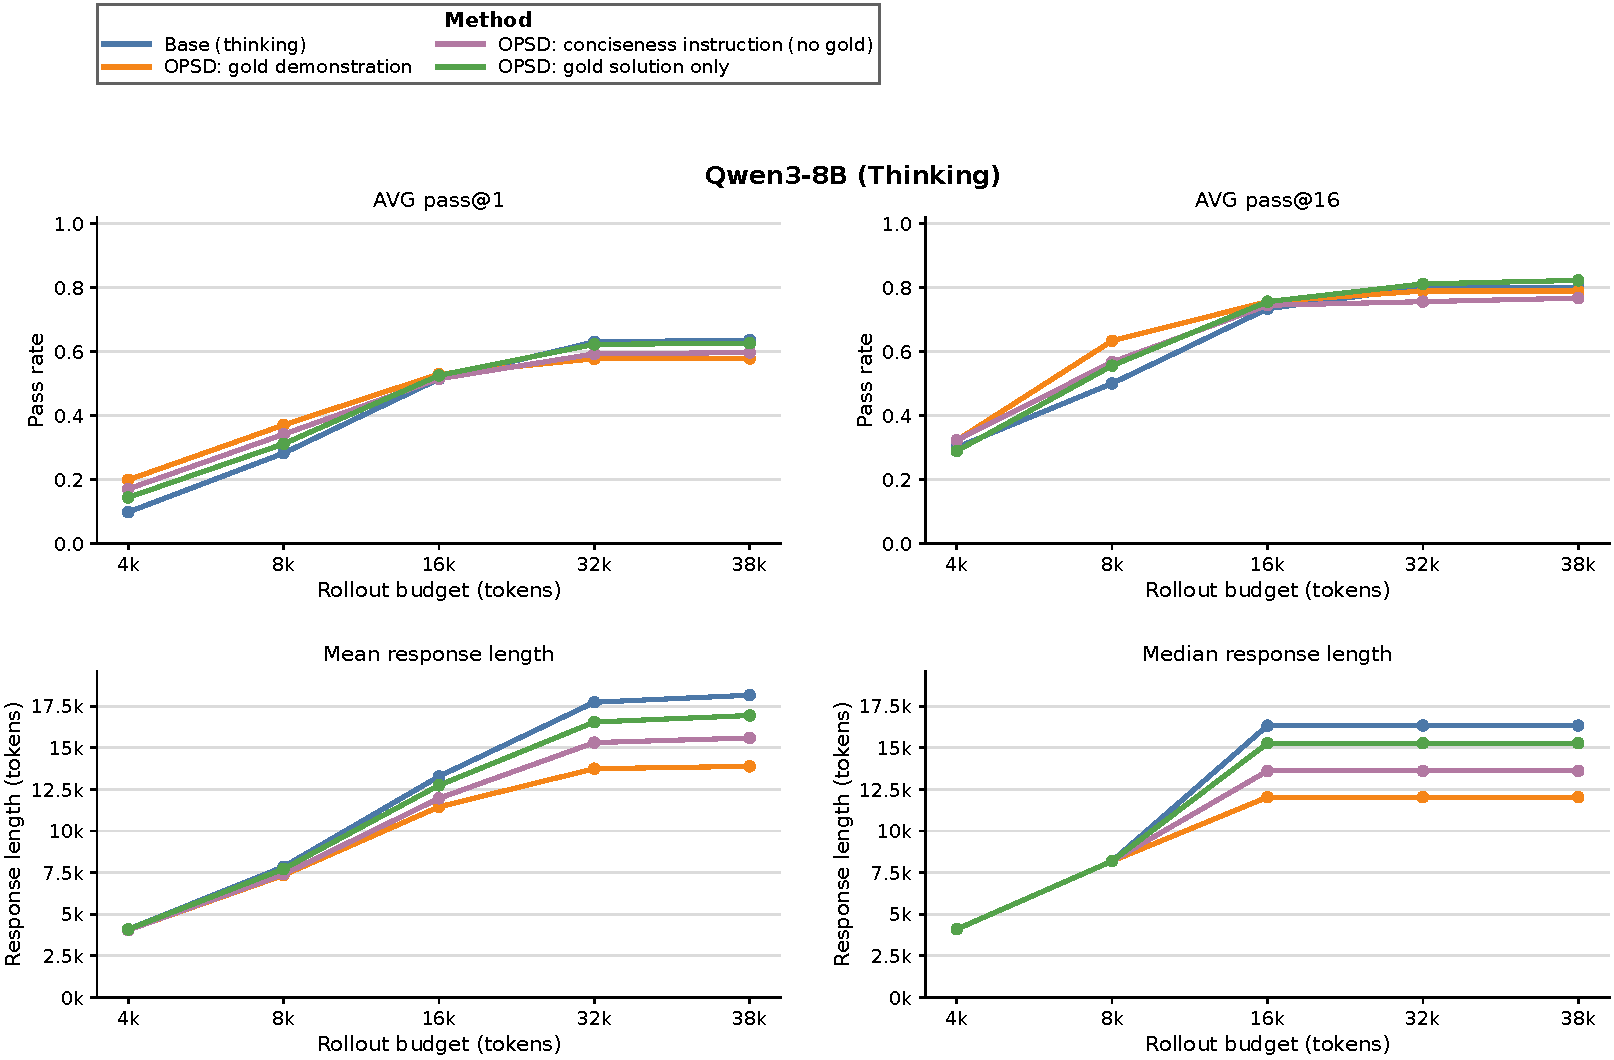
\includegraphics[width=\linewidth]{figures/avg_pass_rollout_qwen8b_with_concise.pdf}
    \caption{
    \textbf{A CRISP-style conciseness prompt compresses Qwen3-8B responses but does not recover the long-budget gains.}
    We compare base \qweneightb{} thinking, \opsd{} with full gold demonstrations, \opsd{} with final-answer-only privileged context, and a conciseness-instruction condition with no gold context, following the CRISP prompt direction of \citep{sang2026policy}.
    Top panels report pass@1 and pass@16 averaged over AIME24, AIME25, and HMMT25; bottom panels report mean and median response length.
    The conciseness condition shortens 32k--38k rollouts relative to the base and gold-solution-only runs but is less compressive than full gold demonstrations.
    Its accuracy follows the same tradeoff: it improves short-budget performance but, at long budgets, remains below the base and gold-solution-only curves, suggesting that making the student concise alone is not enough to preserve the gains from longer thinking rollouts.
    }
    \label{fig:openthoughts_qwen8b_concise_budget}
\end{figure}
